%
% File main.tex
%
% Contact: car@ir.hit.edu.cn, gdzhou@suda.edu.cn
%%e.agirre@ehu.es or Sergi.Balari@uab.es
%% and that of ACL 08 by Joakim Nivre and Noah Smith

\documentclass[11pt]{article}
\usepackage{acl2015}
\usepackage{times}
\usepackage{url}
\usepackage{latexsym}
\usepackage{graphicx}
\usepackage{listings}

%\setlength\titlebox{5cm}

% You can expand the title box if you need extra space
% to show all the authors. Please do not make the title box
% smaller than 5cm (the original size); we will check this
% in the camera-ready version and ask you to change it back.


\title{Spoiler detection and extraction\\Project Report for NLP Course, Winter 2022}

\author{M. Kierznowski, Ł. Pancer, P. Wesołowski \\
  Warsaw University of Technology \\
%   {\tt email@domain} \\
  \And
    supervisor: Anna Wróblewska \\
  Warsaw University of Technology \\
    {\tt anna.wroblewska1@pw.edu.pl}
    }

\date{}

\begin{document}
\maketitle
\begin{abstract}
This document presents the results of the first project for the Natural Language Processing course. The project addresses the spoiler detection task. The topic has not been fully exploited yet in the NLP field. Current research in this field mainly relates to classification without touching the model rationale. After creating the classification models based on pretrained BERT-family architectures, we analyze the model interpretability. Motivated by the ERASER benchmark, we employ the LIME tool and conduct a series of experiments using a precisely annotated dataset. Besides, we extend the previous spoiler detection works by utilizing a large IMDB dataset, hoping for an improvement in performance. The transfer learning using the knowledge from this large dataset is tested in this work. Finally, considering our current achievements, we provide ideas for the next project. 
\end{abstract}

\section{Introduction}

In everyday life, information that reveals the important aspects, events, and twists of a plot of, e.g., a book, a movie, or a videogame is referred to as a spoiler. Spoilers are usually undesired, and getting to know one of them may contribute to a decrease in enjoyment \cite{abbott2020can} or a lack of further interest in reading or seeing the particular position \cite{li2022exploring}. However, they can often become known by chance, for example, due to being a part of some review. Therefore, automatic spoiler detection has become one of the crucial tasks in the NLP field \cite{guo2010finding}.

Several methods on this issue have been proposed. While the authors often focus on their classification performance, we believe that the interpretability aspects are also important and may be an adequate measure of the actual performance. To be specific, examining how the models work internally, what are the rationale behind their decisions, may identify their robustness. Therefore we are going to develop a tool for the assessment of the spoiler classification performance on the basis of the model rationale.

Transfer learning has become popular in recent years due to possible better performance, shorter training time, hence lower electricity usage, or use of other, more readily available data \cite{torrey2010transfer,weiss2016survey}. However, proper fine-tuning on the task-related dataset may be important for further improvement in the model's robustness and accuracy. Similarly to our predecessors, we are going to utilize powerful pre-trained models. However, we would like additionally to make use of the IMDB reviews dataset \cite{enam_biswas_2021}. Although the smaller version is frequently used in the NLP tasks, its much larger variant, which we employ, is rarely utilized. We believe that due to its size (and, therefore, probably its diversity), it may be a good source of additional knowledge for our models.

Our project is driven mainly by two questions: 
\begin{enumerate}
    \item How do the numeric measurements of the model performance (accuracy, ROC AUC) relate to its performance evaluated in a more strict but interpretability-based way? We will compare the accuracy results with our own metrics, which are based on the model rationale.
    \item Does providing a larger task-related dataset for fine-tuning result in the improvement of the spoiler detection model?
\end{enumerate}

The remainder of this work is organized as follows. Section \ref{related-work} provides a brief literature review. Section \ref{datasets} introduces the datasets utilized. Our approach is described in section \ref{approach}. Section \ref{experiments} presents the experiments conducted along with their results. The results obtained are further discussed in section \ref{discussion}. Finally, the conclusions and future work are presented in section \ref{conclusions}.

\section{Related work} \label{related-work}
Spoiler detection tasks had been previously neglected \cite{wan2019fine}, and only in recent years it saw more rapid development. Early studies related to spoiler detection treated it as a traditional classification task, most commonly utilizing methods such as Support Vector Machines. The progress revolved around the process of building a larger dataset with more linguistic features available. The previous works explored basic Bag-of-Words approaches: creating a blacklist of words for a given topic \cite{golbeck2012twitter}, introducing temporal filtering system \cite{nakamura2007temporal}, using topic models based on Latent Dirichlet Allocation \cite{guo2010finding}. Significant contributions to publicly available datasets include TV Tropes Movies \cite{boyd2013spoiler} and Goodreads dataset \cite{wan2019fine}. Chang \shortcite{chang2018deep} proposed an attention-based solution, and today similar approaches still remain state-of-the-art. More recently, a transfer learning approach was suggested, laying the stress on interpretability \cite{wroblewska2021spoiler}.

Regarding the interpretability, the introduction of LIME \cite{lime}, as well as the introduction of SHAP \cite{NIPS2017_7062} are particularly interesting. LIME is an explanation technique designed to explain black-box models, which are common in the NLP field due to the high-dimensional nature of features. It uses a local linear approximation to explain the model's predictions. SHAP is a superset of LIME, basing the explanations on a game theory concept of Shapley values. LIME and SHAP in NLP models enable extracting words that are responsible for making a certain prediction and provide metrics on a strength of their contribution. DeYoung \shortcite{deyoung2019eraser} introduced a benchmark based on datasets with rationales annotated by humans to assess the interpretability of NLP models by comparing their rationales with humans'. This benchmark may be utilized on a custom dataset, provided that it features precise annotations for every class.


\section{Datasets} \label{datasets}
In our research, we have utilized three different datasets. One of them comes in two versions. The overall characteristics of all the datasets used are as follows:
\begin{itemize}
\item Goodreads imbalanced\footnote{available at \url{https://sites.google.com/eng.ucsd.edu/ucsdbookgraph/home}} - 1.3M documents, 17M sentences, 570k spoiler sentences, 1:15 spoiler to non-spoiler reviews ratio,
\item Goodreads balanced\footnote{available at \url{https://spoiler-datasets.s3.eu-central-1.amazonaws.com/goodreads_balanced-[train, val, test].json.gz}} - 180k documents, 3.1M sentences, 570k spoiler sentences, 1:1 spoiler to non-spoiler reviews,
\item TV Tropes Books\footnote{available at \url{https://github.com/rzepinskip/tvtropes-books}} - 340k documents, 670k sentences, 110k spoiler sentences, 1:4 spoiler to non-spoiler reviews,
\item IMDB reviews\footnote{available at \url{https://www.kaggle.com/dsv/1836923}} - 5.5M documents, 1:4 spoiler to non-spoiler reviews ratio.
\end{itemize}
One can see that the default Goodreads is highly imbalanced. That's why during the training procedure, we use its balanced version.

The datasets offer different levels of annotations. Our task is focused on document classification, but additional annotations are used for interpretability investigation.
The Goodreads dataset provides sentence-level spoiler annotations, i.e., each sentence is marked either as a spoiler or a non-spoiler. The TV Tropes Books is the more precise one since it offers word-level spoiler annotations. Finally, the IMDB dataset is the largest one. However, it provides only document-level annotations. Samples from these three datasets are presented in listings \ref{lst:sample-goodreads}, \ref{lst:sample-tvtropes-books}, \ref{lst:sample-imdb} respectively.

Further exploratory data analysis is provided in section \ref{eda}.

\begin{figure*}[h]
\begin{lstlisting}[basicstyle=\small,caption={Sample JSON object in the Goodreads dataset. Each sentence contains an integer flag that identifies spoiler sentences. Note that some entries were truncated due to readability reasons.},label={lst:sample-goodreads}]
{
'user_id': '1ceef4796fb36190e72714895806835b',
'timestamp': 1445212800000,
'review_sentences': [[0, 'When I read through this ...'],
    [1, 'She jerked around two really great guys...'], ...],
'rating': 3,
'has_spoiler': True,
'book_id': 18304322,
'review_id': '9e7cc14cc03b22a88875a21195e58454',
'genres': {'young-adult': 1763, 'romance': 438, 'fiction': 885}
}
\end{lstlisting}

\begin{lstlisting}[basicstyle=\small,caption={Sample JSON object in the TV Tropes Books dataset. Each sentence contains a boolean flag that identifies spoiler sentences. In addition, annotated character indices provide specific spoiler boundaries.},label={lst:sample-tvtropes-books}]
{
'page': 'https://tvtropes.org/...',
'trope': 'Kill the Cutie',
'has_spoiler': True,
'sentences': [[True, 'Walter, who was the ...', [[0, 89]]]]
}
\end{lstlisting}

\begin{lstlisting}[basicstyle=\small,caption={Sample JSON object in the IMDB dataset. The dataset features only document-level annotations},label={lst:sample-imdb}]
{
'review_id': 'rw1133942',
'reviewer': 'OriginalMovieBuff21',
'movie': 'Kill Bill: Vol. 2 (2004)',
'rating': 8.0,
'review_summary': 'Good follow up that answers all the questions',
'review_date': '24 July 2005',
'spoiler_tag': 0,
'review_detail': "After seeing Tarantino's Kill Bill Vol: 1, I ...",
'helpful': ['0', '1']
}
\end{lstlisting}

\end{figure*}





\section{Approach} \label{approach}

In general, our methodology consists of the following points:
\begin{itemize}
\item Train the document classification models for three datasets separately.
\item Examine the transfer learning performance using the IMDB model on two other datasets.
\item Verify the rationale behind the models using precisely annotated TV Tropes Books dataset. The custom metric is proposed in this step.
\end{itemize}

In line with the approach proposed by Wróblewska \shortcite{wroblewska2021spoiler}, we have focused on state-of-the-art solutions based on transformer architecture. Namely, our current classifiers have been built on BERT-based architectures. Apart from exploring the standard BERT Base-uncased model, we decided to try smaller DistilBERT architecture. Due to our computational limits, we felt it would be better to go this way rather than larger models such as the ELECTRA. According to the original paper, DistilBERT has 40\% fewer parameters than BERT Base-uncased and offers 60\% speedup. Table \ref{tab:bert-comparison} shows a more exact comparison.

\begin{table}[h]
    \centering
    \begin{tabular}{|c|c|}
        Model & \#Parameters \\\hline
        DistilBERT & 66M \\
        BERT & 110M
    \end{tabular}
    \caption{Comparison of used BERT-based base architectures}
    \label{tab:bert-comparison}
\end{table}

On top of the base architecture, we use a single fully-connected linear layer preceded by a dropout. Pooled BERT outputs serve as input for the dropout layer and final classification head. Because of the potential time advantages of DistilBERT, in addition to accuracy scores, we also compare the running times of the two models. We verify whether it agrees with expectations and what the impact is on performance results.


IMDB dataset contains a substantially greater amount of sentences than the other collections. We decided to test whether the generalizations learned by training on this dataset can be transferred. To do that, we conduct experiments in which we utilize weights from IMDB training. In total, two sets of experiments are conducted. In the primary experiments, we evaluate the IMDB-trained BERT model, without any adjustments, on Goodreads balanced and TV Tropes Books test sets. In the next stage, we examine fine-tuning the model further using the respective training sets for one epoch with different values of learning rate. For this purpose, the BERT layers are frozen, and only the parameters of the last dense layer remain trainable.

Some explainable artificial intelligence method is needed for the explanation of chosen models. In the preliminary report, two methods were considered: LIME and ERASER. Unfortunately, implementing ERASER for a dataset different than stated in the paper is complicated and requires human rationale for all classes. Due to this fact, LIME is a better suits our needs of examining the model and finding words that the model indicates as spoilers. In the source code of our experminets we utilized the most popular Lime implementation on Python Package Index\footnote{available at https://github.com/marcotcr/lime}. The application of LIME has been made on the TV Tropes Books dataset because it features word-based annotations. This fact gives the possibility to compare indicated words to actual spoilers annotated by the creators of the dataset.
Before computing the LIME metrics, some parameters need to be chosen:

\begin{itemize}
    \item  numfeatures: which stands for the maximum number of features present in the explanation. During the research, this parameter was set to 10. Bigger values tend to catch non-informative words such as (a, the, or an),

    \item numsamples: which stands for the size of the neighborhood to learn the linear model (number of perturbated examples). During the research, this parameter was set to 1500. More significant values tend to highly increase the time of calculation without any additional value.
\end{itemize}

While LIME explains the instance, it perturbates input (according to numsamples parameter) and compares probabilities between the classes. Finally, it aggregates the data from all of the perturbated instances computing the final LIME score. An example of LIME explaining an instance is shown in figure \ref{fig:LIMEexample}.

\begin{figure}[h]
    \centering
    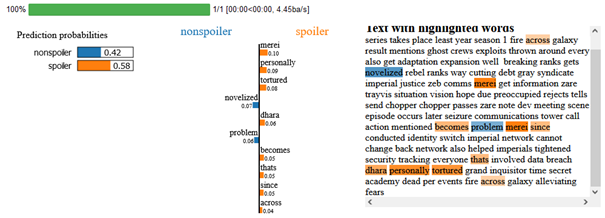
\includegraphics[width=\columnwidth]{img/Obraz1.png}
    \caption{Example of LIME} 
    \label{fig:LIMEexample}
\end{figure}

Before executing the script, stop words have been cut out from the instance. Otherwise, sometimes they would appear with positive contribution, but as we know, words such as “a” do not reveal any information about the story. The figure~\ref{fig:LIMEexample} lists words: merei, personally, tortured, Dhara, that's, since, and across. They have the biggest contribution to the classification of this instance as a spoiler. Words such as tortured or Dhara (Name) reveal some information about the storyline. Thus it is a confirmation that created models can distinguish words. However, accessing our model on a single instance is impossible. Because of that, some additional metrics have been created.
\begin{itemize}
    \item Sentence-based statistics. Sum up LIME within a sentence such that we choose sentences with the highest score.
    \item Additionally, we compute word-based statistics by comparing sets of words indicated by LIME and actual spoilers.
\end{itemize}

In order to calculate LIME, we sum up the LIME metrics into sentences (omitting negative values). Then we select sentences with the highest aggregated sum and compare them with the actual spoiler sentences. For example, the document consists of four sentences 1, 2, 3, and 4 (where 3 and 4 are actual spoilers). Suppose we aggregated LIME metrics per all sentences, and it turns out that sentences 1 and 3 are indicated as a spoiler. Then they are compared with actual spoilers, and if at least one indicated sentence is present in actual spoilers, value "1" is assigned and "0" otherwise. 


\section{Experiments and results} \label{experiments}
\subsection{Exploratory data analysis} \label{eda}


\subsubsection*{Goodreads}
This data set may be found in two forms: balanced, which is used in provided research, and standard. We have selected the balanced alternative in order to provide research on at least one balanced dataset.

For the spoiler sentences (assigned to accommodate spoilers), the frequency distribution of words is provided in figure \ref{fig:freq-dist}. Note that before calculations, stop words were deleted (downloaded from the nltk package) as well as punctuation marks such as "," or ".".

\begin{figure}
    \centering
    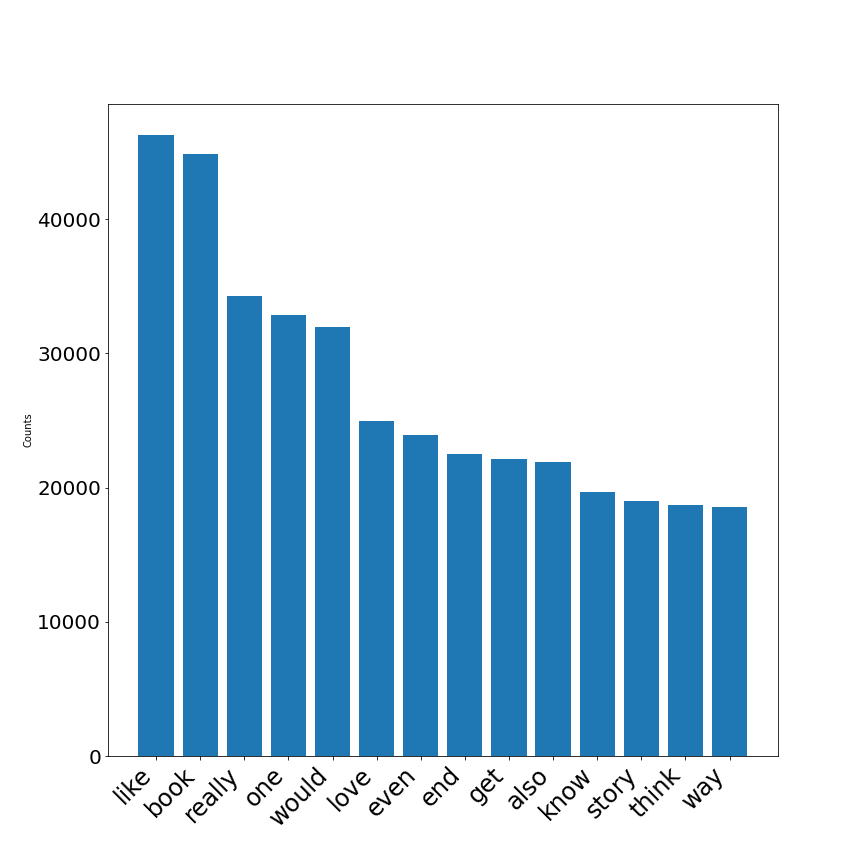
\includegraphics[width=\columnwidth]{img/FreqDistFiqure.png}
    \caption{Frequency Distribution of sentences containing spoiler for Goodreads dataset}
    \label{fig:freq-dist}
\end{figure}

Analyzing provided figure, we can presume that words such as \emph{love}, \emph{know}, or \emph{story} may hold undesirable content.

Finally, one important issue is worth elaborating on. We focus on the whole review classification. Moreover, our models are BERT-based, which means they can handle up to 512 input tokens. The reviews where the first spoiler occurs after the first 512 tokens may be problematic. We investigated this topic further and estimated that about 90\% of spoiler reviews contain at least one spoiler within the first 512 tokens. Therefore, we decided to leave it as it is. Besides, who knows if the model cannot learn if the review contains spoilers on the basis of only part of it? (using, e.g., the author's writing style, etc.).

\subsubsection*{TV Tropes Books}

This dataset provides more detailed information about spoilers. It also contains word-based information, i.e., which specific words are spoilers. Applying frequency distribution of words among spoilers sentences provides compelling information about specific words, as shown in figure~\ref{fig:freq-dist-troop}.

\begin{figure}
    \centering
    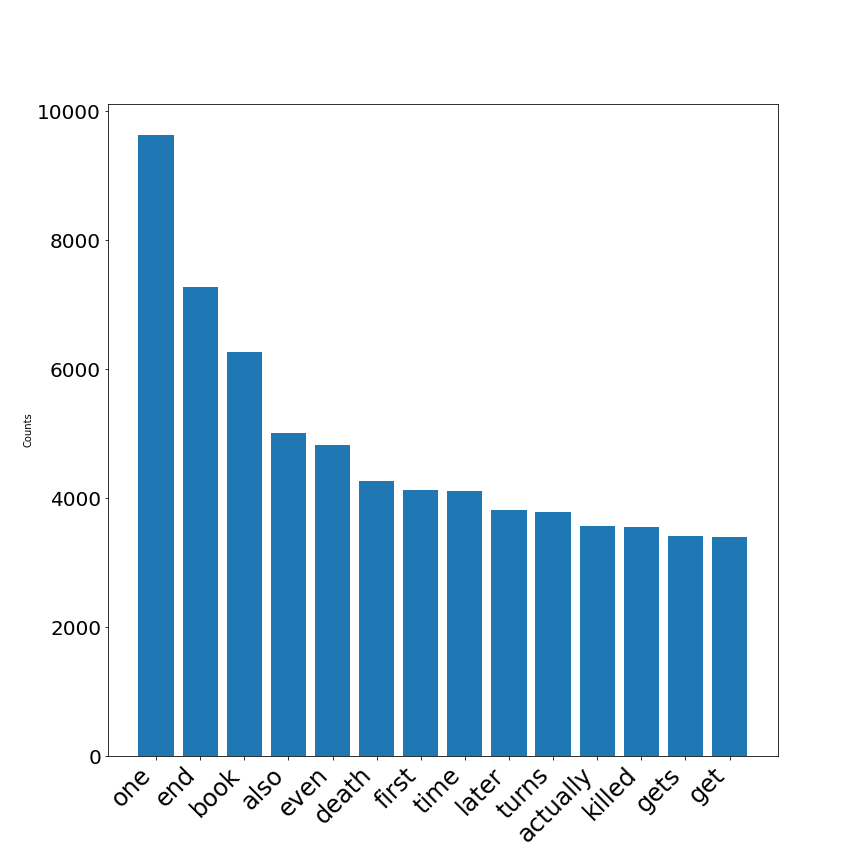
\includegraphics[width=\columnwidth]{img/FreqDistFiqure_Troops.png}
    \caption{Frequency Distribution of sentences containing spoiler for TV Tropes Books dataset} 
    \label{fig:freq-dist-troop}
\end{figure}

Figure \ref{fig:freq-dist-troop} reveals words that may strongly contribute to spoilers, such as \emph{death} or \emph{killed}. Looking closer at those trigger words may contribute to finding some specific pattern. 

\subsubsection*{IMDB reviews}
Contrary to the other two datasets, the IMDB reviews set contains only document-level annotations. Therefore, we cannot extract as much information from this dataset as in previous cases.

The dataset is highly imbalanced, as shown in figure \ref{fig:imdb-classes}. It features roughly 1.2M non-spoiler reviews and 4.4M spoiler-tagged reviews.

Regarding review lengths, there are 32 outliers containing more than 200 sentences. There are 625 reviews which consist of more than 100 sentences. Figure \ref{fig:imdb-sentence-hist} shows a histogram of review length in terms of the number of sentences. Note that reviews featuring more than 100 sentences are not included. One can see that the vast majority of sentences are shorter ones, with less than 20 sentences.

Due to the very high volume of this dataset, we decided to remove randomly excessive reviews without spoilers to obtain a balanced dataset. We are aware that more sophisticated techniques may be used to deal with this problem, including class weighting or data augmentation. Since the dataset size results in a very long learning time, reducing both was desirable for us.


\begin{figure}[h]
    \centering
    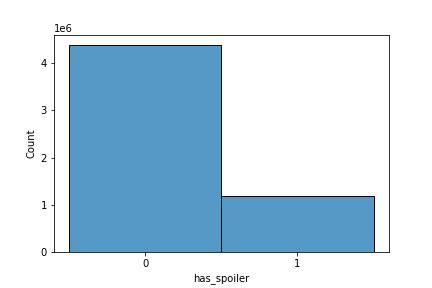
\includegraphics[width=\columnwidth]{img/imdb_classes.jpg}
    \caption{Class distribution in the IMDB dataset}
    \label{fig:imdb-classes}
\end{figure}

\begin{figure}[h]
    \centering
    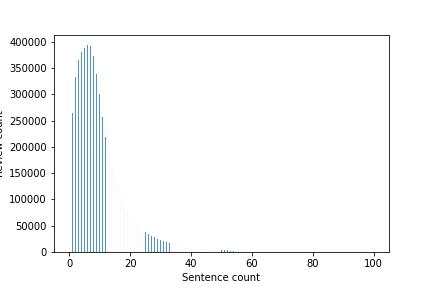
\includegraphics[width=\columnwidth]{img/imdb-sentence-length-hist.jpg}
    \caption{Histogram of review lengths, reviews with more than 100 sentences are not included}
    \label{fig:imdb-sentence-hist}
\end{figure}


\subsection{Training the models}
During our experiments, we utilized the Transformers library \cite{wolf2020transformers}, which provided the models. Our initial experiments were conducted without the penultimate dropout layer, but we observed overfitting, so that's why we included it in further models. Additionally, we used pre-trained weights for BERT-based models.

First, we experimented with all the weights frozen except for the classification head. However, the results achieved in this way were not satisfactory since almost no improvement during the training was observed. That's why we decided to optimize all the weights of our models.

\subsubsection*{Goodreads}

For the Goodreads dataset, we tested both DistilBERT as well as BERT models. 
The dataset was already split into train, test, and validation datasets. Each part was tokenized and converted to the TensorFlow Dataset class. It turned out that the training process took a long. Therefore, we have managed to train DistilBERT and BERT classifiers only for 3 epochs. The final dropout was set to 0.1. The initial learning rate was set to 2e-5 and followed by linear decay with Adam optimizer. Both models were trained using the balanced dataset and evaluated on both the balanced and entire datasets. We have taken care to remove from the full dataset entries that were used to train the model.

The results for both the balanced test set and imbalanced test set are provided in tables \ref{tab:goodreads-balanced-results} and \ref{tab:goodreads-imbalanced-results}. We also present previous works' results, where applicable.
Let us stress again that in the presented experiments, all model weights were optimized.


\begin{table}[h]
    \centering
\begin{tabular}{|l|l|l|l|}
\hline
\begin{tabular}[c]{@{}l@{}}Classifier\\ architecture\end{tabular} & Accuracy & ROC AUC & F1     \\ \hline
BERT                                                              & 0.8196   & 0.9037  & 0.8171 \\ \hline
DistilBERT                                                        & 0.8144   & 0.8990  & 0.8144 \\ \hline
\end{tabular}
    \caption{Results achieved for the balanced Goodreads reviews test set}
    \label{tab:goodreads-balanced-results}
\end{table}

\begin{table}[h]
    \centering
\begin{tabular}{|l|l|l|l|}
\hline
\begin{tabular}[c]{@{}l@{}}Classifier\\ architecture\end{tabular} & Accuracy & ROC AUC & F1     \\ \hline
BERT                                                              & 0.8289   & 0.9019  & 0.0646 \\ \hline
DistilBERT                                                        & 0.8100   & 0.8947  & 0.0588 \\ \hline
\begin{tabular}[c]{@{}l@{}}Wróblew-\\ ska et al.\\ \shortcite{wroblewska2021spoiler}\end{tabular}   &          & 0.8821  &                                                                    \\ \hline
\begin{tabular}[c]{@{}l@{}}Wan et al.\\ \shortcite{wan2019fine}\end{tabular}
 &          & 0.9190  &                                                                    \\ \hline
\end{tabular}
    \caption{Results achieved for the whole imbalanced Goodreads reviews test set along with reference solutions}
    \label{tab:goodreads-imbalanced-results}
\end{table}


\subsubsection*{TV Tropes Books}

\begin{table*}[t]
    \centering
\begin{tabular}{|l|l|l|l|l|}
\hline
\begin{tabular}[c]{@{}l@{}}Classifier\\ architecture\end{tabular} & Accuracy & ROC AUC & F1     & \begin{tabular}[c]{@{}l@{}}Balanced\\ accuracy\end{tabular} \\ \hline
BERT                                                              & 0.8507   & 0.8750  & 0.6166 & 0.7415                                                      \\ \hline
DistilBERT                                                        & 0.8439   & 0.8670  & 0.5829 & 0.7208                                                      \\ \hline
Wróblewska et al. \shortcite{wroblewska2021spoiler}  &          & 0.8471  &        &                                                             \\ \hline
\end{tabular}
    \caption{Results achieved for the TV Tropes Books reviews test set along with reference solution}
    \label{tab:tropes-results}
\end{table*}

% Due to plans of combining the datasets to create a more general model, we decided on classifying the entire documents of TV Tropes as opposed to classifying individual sentences to either contain a spoiler or not. Such an approach slightly improves the balance of the dataset from 16\% of spoiler-tagged reviews to 22\%, which still makes a greatly imbalanced dataset.
Not having access to a balanced version of the TV Tropes Books, we decided to account for the difference using class weights, which proved difficult due to the implementation of selected models and was ultimately discarded. Augmentation of TV Tropes is another solution for the problem of imbalance to consider. Nevertheless, we conducted a training on TV Tropes Books without accounting for imbalance, using the same configuration as for the previous dataset.

The results of the experiments are shown in table \ref{tab:tropes-results}. Due to the class imbalance, we also included balanced accuracy.




\subsubsection*{IMDB}
As mentioned before, we carried out a single experiment using a balanced IMDB dataset. It contained roughly 2.4M reviews, with half of it marked as spoilers. We split this balanced version into train, validation, and test parts in proportions of 0.8, 0.1, and 0.1.
Due to recurring training time issues, particularly pronounced in the case of IMDB, we used the same configuration of 3 epochs, final dropout set to 0.1, and Adam optimizer with decaying learning rate, starting from 2e-5. We saved the weights after the second epoch because the validation results were better compared to the end of the training.

Table \ref{tab:imdb-results} shows the results achieved on the test set. Here, we measured only the accuracy and balanced accuracy. Note that we didn't repeat the experiments, i.e., it was conducted only once. That's due to the learning time. We have not measured the other metrics, but even the interference was taking a lot of time, and we couldn't repeat the experiment.

\begin{table}[h]
    \centering
\begin{tabular}{|l|l|l|}
\begin{tabular}[c]{@{}l@{}}Classifier\\ architecture\end{tabular} & Accuracy & \begin{tabular}[c]{@{}l@{}}Balanced\\ accuracy\end{tabular} \\ \hline
BERT                                                              & 0.7782   & 0.7783                                                     
\end{tabular}
    \caption{Results achieved for the IMDB reviews test set}
    \label{tab:imdb-results}
\end{table}


In addition to the previous measurements, in the case of all the datasets (Goodreads, TV Tropes Books, IMDB), we also measured the training and inference times. Since our calculations were conducted on different machines, we do not provide the exact measurements since not to suggest their comparison between data sets. However, in all cases, the training of the DistilBERT architecture was roughly 2 times faster than BERT. Regarding the inference, DistilBERT proved to be $2.1$ times faster than its larger variant.

\subsection{Transfer learning with BERT trained on the IMDB dataset}

In the first set of experiments, we evaluated the IMDB model on the remaining datasets. The IMDB model was not fine-tuned in both cases. The subsequent set of experiments consisted of fine-tuning the IMDB model on the datasets to be evaluated. Only the last classification layer was fine-tuned for one epoch with different learning rates. Tables \ref{tab:goodreads-imdb-lr} and \ref{tab:tv-tropes-imdb-lr} contain results for Goodreads and TV Tropes Books datasets, respectively. Apart from the results achieved using the IMDB-trained model, the scores from the previous experiments are also provided.
 

% \begin{table}[h]
%     \centering
% \begin{tabular}{|l|l|l|l|}
% Model & Accuracy & ROC AUC & F1 \\ \hline
% \begin{tabular}[c]{@{}l@{}}IMDB\\ Model\end{tabular}                                                                & 0.7623   & 0.8442  & 0.79 \\
% \hline
% \begin{tabular}[c]{@{}l@{}}Goodreads\\ Model\end{tabular}                                                        & 0.8196   & 0.9037  & 0.8171
% \end{tabular}
%     \caption{Results achieved on the Goodreads reviews test set, IMDB model was not fine-tuned}
%     \label{tab:goodreads-imdb-lr-no}
% \end{table}

% \begin{table}[h]
%     \centering
% \begin{tabular}{|l|l|l|l|}
% Model & Accuracy & ROC AUC & F1 \\ \hline
% \begin{tabular}[c]{@{}l@{}}IMDB\\ Model\end{tabular}                                                            & 0.6256   & 0.7581  & 0.47 \\
% \hline
% \begin{tabular}[c]{@{}l@{}}TV Tropes\\ Model\end{tabular}                                                      & 0.8507   & 0.8750  & 0.6166
% \end{tabular}
%     \caption{Results achieved on the TV Tropes Books reviews test set, IMDB model was not fine-tuned}
%     \label{tab:tv-tropes-imdb-lr-no}
% \end{table}






\begin{table}[h]
    \centering
\begin{tabular}{|l|l|l|l|}
\begin{tabular}[c]{@{}l@{}}Learning\\ Rate\end{tabular}  & Accuracy & ROC AUC & F1 \\ \hline

\begin{tabular}[c]{@{}l@{}}No\\ finetuning\end{tabular}  & 0.7623   & 0.8442  & 0.79 \\\hline

0.0002                                                              & 0.7622   & 0.8442  & 0.79 \\
\hline
0.002                                                              & 0.7748   & 0.8550  & 0.78 \\
\hline
0.02                                                              & 0.7772   & 0.8619  & 0.78 \\
\hline
\begin{tabular}[c]{@{}l@{}}Goodreads\\ model\end{tabular}                                                        & 0.8196   & 0.9037  & 0.8171
\end{tabular}
    \caption{Results achieved on the Goodreads reviews test set for IMDB model fine-tuned with a corresponding learning rate and the previous model}
    \label{tab:goodreads-imdb-lr}
\end{table}


\begin{table}[h]
    \centering
\begin{tabular}{|l|l|l|l|}
\begin{tabular}[c]{@{}l@{}}Learning\\ Rate\end{tabular}    & Accuracy & ROC AUC & F1 \\ \hline

\begin{tabular}[c]{@{}l@{}}No\\ finetuning\end{tabular} & 0.6256   & 0.7581  & 0.47 \\
\hline

0.0002                                                           & 0.6256   & 0.7581  & 0.47 \\
\hline
0.02                                                           & 0.6333   & 0.7672  & 0.49 \\
\hline
\begin{tabular}[c]{@{}l@{}}TV Tropes\\ model\end{tabular}                                                      & 0.8507   & 0.8750  & 0.6166
\end{tabular}
    \caption{Results achieved on the TV Tropes Books reviews test set for IMDB model fine-tuned with a corresponding learning rate and the previous model}
    \label{tab:tv-tropes-imdb-lr}
\end{table}


\subsection{Explainability}

The following tables represent gathered results for the explainability. The second column of the table \ref{tab:sentence-based-comparison} shows the mean for the calculation of presence of a sentence in the spoiler set. In the third column, we compared sets such that, according to the previous example, we counted mutual examples and divided them by the number of sentences (3 are mutual, so the statistic is 0.25). 



\begin{table}[h]
    \centering
    \begin{tabular}{|c|c|c|}
    \begin{tabular}[c]{@{}l@{}} Sentence \\Based \end{tabular}  & \begin{tabular}[c]{@{}l@{}} At least one\\ sentence in spoiler\\ sentences \end{tabular} & \begin{tabular}[c]{@{}l@{}} Set \\ comparison\end{tabular} \\\hline
        % Sentence Based & At least one sentence in spoiler sentences & Set comparison \\\hline
        BERT & 16\% & 6\% \\
        DistilBERT & 16\% & 6\% 
    \end{tabular}
    \caption{Sentence based metrics}
    \label{tab:sentence-based-comparison}
\end{table}


Unfortunately, sentence-based metrics are relatively low for both models. It means that our model cannot correctly distinguish sentences containing spoilers.

Word-based metrics represents a different view, where we calculate LIME for ten words, and the comparison between actual spoilers has been made. Then we select 10, 5, or a single word with the biggest contribution. Results are shown in table \ref{tab:wordbased}.

\begin{table}[h]
    \centering
    \begin{tabular}{|c|c|c|c|}
    \begin{tabular}[c]{@{}l@{}@{}} Word \\Based \end{tabular}  & \begin{tabular}[c]{@{}l@{}} Top 10\\ words \end{tabular} & \begin{tabular}[c]{@{}l@{}} Top 5\\ words \end{tabular} &
    \begin{tabular}[c]{@{}l@{}@{}} Top 1\\ word \end{tabular} \\\hline
        
        % Word based & Top 10 words & Top 5 words & Top 1 word \\\hline
        BERT & 89\% & 84\%  & 31\% \\
        DistilBERT & 87\% & 84\%  & 35\% 
    \end{tabular}
    \caption{Word based metrics}
    \label{tab:wordbased}
\end{table}


Moreover, it turns out that in the top 5 words, there is an 84\% chance that at least one actual spoiler is within the set. Furthermore, Distil Bert has a 35\% chance that the word with the highest score is an actual spoiler (Note that the number of words for a document often reaches 100 distinct words).

The second column shows the mean of that calculation. In the third column, we compared sets such that, according to the previous example, we counted mutual examples and divided them by the number of sentences (3 are mutual, so the statistic is 0.25).


\section{Discussion} \label{discussion}

Considering the Goodreads balanced dataset, we can see that the classification models created performed well. However, it's due to the optimization of all the model parameters, which is time-consuming. The situation changes when we look at the imbalanced test version of the dataset. While the accuracy and ROC AUC scores remain similar, there is a significant drop in F1. We have investigated the reason, and it turned out that the precision was very low. It means that the model identified many non-spoiler reviews as spoilers. Note that such an outcome could be expected. The imbalanced data contains about 15 non-spoilers for a single spoiler, so any errors are often related to the misclassification of non-spoilers. In addition, the model was trained using balanced data. If the model somehow memorized the apriori probabilities (which might have been significant in case of ambiguity), they were not valid anymore. The results obtained show the importance of measuring the F1 scores in this type of classification.

The results achieved are comparable to the reference ones. However, we have found only the ROC AUC scores in other works, so we do not believe that this comparison is conclusive. In addition, we were not able to repeat our experiments due to the computational complexity, so they may not be statistically significant.

When it comes to the TV Tropes Books dataset, the results show some issues related to class imbalance, similar to the previous dataset. Both the training and testing subset of TV Tropes Books expose a similar imbalance level with about 4 non-spoilers for a single spoiler. In this case, we also encountered a precision decrease. Comparison with the reference score may indicate that we managed to train a better model. However, without the other metrics, including F1, we would like to refrain from such statements.

We have only accuracy measurements reported for the IMDB dataset, and they aren't promising when compared to other datasets. However, it was not our goal to build a powerful IMDB classifier. We simply wanted to have a model pretrained on a large IMDB dataset for further fine-tuning on other data.


Regarding the DistilBERT vs. BERT comparison, the lighter model with a significantly smaller number of parameters achieved only slightly worse results. Taking into account the fact that it offers 2x speedups, we consider it an attractive alternative.

Regarding the evaluation of the IMDB model performance on the other datasets, in both instances, the model performed poorer than the models trained on corresponding training datasets.
After additional last layer fine-tuning, the outcome did not differ significantly from the initial values, with slightly better results obtained for larger learning rates.
The results of these experiments prove that it might be difficult to develop a universal solution for detecting all kinds of spoilers. We conclude that the nature of spoilers differs between the datasets, and our models have not extracted patterns that are general enough to be successfully used on different datasets. We believe that for that purpose, a model would have to be trained on data from various sources, with spoilers from diverse media types.


\section{Conclusions and future work} \label{conclusions}


Overall we are very much satisfied with the results, as all experiments were successfully carried out and yielded conclusive results. For the models trained on specific datasets we have managed to obtain a slight improvement over the state-of-the-art results and complemented them with additional metrics, which were not present in the majority of previous scientific papers on the spoiler detection topic. We consider them to be crucial to properly interpret the viability of the results, and we believe that future researchers might benefit from that inclusion. The transfer learning experiments, while turned out with negative results, provided a deeper insight into the problem domain, and gave directions to the next potential research topics.

The explainability analysis showed that the models differentiate between spoiler and non-spoiler words. Applying the LIME method confirms that models can detect words containing information about the story. The mentioned case scenario provides information that some words correctly trigger model answers and contribute to a a piece of text being a spoiler. However, aggregations of sentence-based and word-based metrics show that a single LIME method incorporated into BERT is insufficient to detect all spoilers correctly. Furthermore, it's hard to find some aggregate metrics for LIME to correctly generalize the score over the whole dataset. Thus we are not ensured that our metrics provide accurate information about generalized model responses.

% W tym pierwszym pomysle trzebea wymienic spodziewane problemy, tj. brak literatury, wzrost zlozonosci obliczeniowej jak na wyjsciu jest duzo outputow

Our first main idea for the next project would be to utilize the precise annotations provided in the TV Tropes Books dataset. Namely, we would like to create a model which can predict which specific words may be considered a spoiler (something like phrase extraction). We have not found any literature on such a topic, except for a Kaggle contest \url{https://www.kaggle.com/c/tweet-sentiment-extraction} and a sample solution \url{https://medium.com/analytics-vidhya/tweet-sentiment-extraction-e5d242ff93c2}. An approach would be to treat this task as a classification task with many outputs, each corresponding to a single word. However, since the computational complexity of such a model increases, it may be hard to implement and test. Additionally, as already mentioned, we have no literature since we do not know how this task is actually called.

Due to the expected number of problems with our first idea, if we fail to implement it, we will consider a different project. Because the reproducibility of the work is an important issue, we would like to focus on reproducing the SpoilerNet paper \cite{wan2019fine}. We are aware that some attempts have already been carried out but to no avail. Still, the authors reported having achieved a state-of-the-art score. The SpoilerNet architecture utilizes the hierarchical attention network (HAN) \cite{yang2016hierarchical}. The novel idea in SpoilerNet is the incorporation of word frequency information, namely document frequency, and inverse item frequency, into the word embeddings. Even if we fail to reproduce the original results, such a project may be valuable for us since we have no prior HAN architecture experience. 


Division of work:
\begin{itemize}
    \item \textbf{Mateusz Kierznowski} - Explainable Artificial Intelligence, LIME, parts of report and presentation,
    \item \textbf{Łukasz Pancer} - TV Tropes Books model, transfer learning with BERT trained on the IMDB dataset, parts of report and presentation,
    \item \textbf{Paweł Wesołowski} - Goodreads model, IMDB model, parts of report and presentation.
\end{itemize}
Our hourly workload was comparable. It's hard to determine the time-consumption of the project because of the teaching procedures and the use of time for other activities. However, we estimate that the project took about 60 hours.


% include your bib file like this:
\bibliographystyle{acl}
\bibliography{bibliography}

\end{document}